\documentclass{article}
\usepackage{graphicx}
\begin{document}
 
 \title{Metaheurísticas. Trabajo de Evaluación}
\author{Frédéric Roux, PhD}

\maketitle
 
  \section{Problema de la asignación cuadrática y problema de la partición del grafo}
El problema de asignación cuadrática (QAP) y el problema de la partición de un grafo pertenecen al campo de la optimización combinatoria [1-2]. Los dos problemas son problemas computacionales complejos dicho de tipo "NP-hard", es decir se requieren algoritmos no-deterministas basados en heurísticas para encontrar una solución aproximada, ya que una solución exacta de este tipo de problema no es factible en tiempo computacional polynomial [3-4].

\subsection{Descripción del problema de asignación cuadrática (QAP) }
El QAP fue introducido por Koopmans y  Beckman en 1957 en el contexto de la localización de actividades económicas indivisibles [5-6]. El problema consiste en asignar un conjunto de n instalaciones a un conjunto de n localizaciones de manera que se minimize el coste de utilización de las instalaciones. El coste de utilización entre dos instalaciones es dado por la suma del flujo entre estas instalaciones multiplicado por la distancia entre sus localizaciones asignadas. Si denotamos por $\sigma$ = ($\sigma$(1),$\sigma$(2),...,$\sigma$(n)) una posible asignación, y por $f_{kl}$  el flujo entre las instalaciones $k$ y $l$, y por $d_{ij}$ la distancia entre las instalaciones $i$ y $j$, el objetivo del QAP es de minimizar la función objetiva dado por:\newline

 \begin{equation}
	f(\sigma)=\sum_{i=1}^{n}\sum_{j=1}^{n}f_{ij}d_{\sigma(i)\sigma(j)}
\end{equation}

\subsection{Descripción del problema de la bi-partición de grafo}
El problema de partición de grafo pertenece al campo de los problemas de partición y puede ser resumido por el ejemplo sencillo siguiente [7]: dado un conjunto de enteros 2 10 3 8 5 7 9 5 3 2, cual es la partición del conjunto $S$ de enteros que resulta en dos conjuntos $S1$ y $S2$ con sumas iguales? Un ejemplo de partición posible seria $S1$ = 2 5 3 10 7 y $S2$ = 2 5 3 9 8 dado que la suma de cada conjunto es 27 [6]. En el caso del problema de la bi-partición del grafo (BIPART), el problema consiste en particiónar un grafo no dirigido G = ($\chi$,U) con $\chi$ $\neq$ $\emptyset$ y U = \{($u$,$v$) $\mid$ $u$,$v$ $\in$ $\chi$\} en el que cada arista ($u$,$v$) tiene asociado un peso $p(_{u,v})$ y el numero de vertices es par en dos particiones. Por lo tanto, en el problema BIPART se trata de dividir el conjunto de vértices en dos subconjuntos $S1$ y $S2$ iguales, de forma que se minimize la suma de los pesos asociados a aristas que unen vértices de diferentes conjuntos. El objetivo del problema de partición de un grafo es de maximizar la función objetiva dado por:\newline

 \begin{equation}
	f(G)=\sum_{i=1}^{n}p_{ij}
\end{equation}

 \section{Propuesta de solución basada en búsqueda local}
 Con el objetivo de aproximar soluciones para el problema QAP y el problema BIPART, el trabajo presente ha utilizado como primer enfoque metaheuristicas dichas "sin memoria" (memory-less). Mas concretamente, para resolver el problema QAP se ha utilizado la búsqueda local con multiarranque, mientras que para resolver el problema BIPART se ha utilizado el greedy randomized adaptive search procedure (GRASP).\newline
 
En el trabajo presente, la búsqueda local se ha implementado según los pasos descritos en el pseudo-codigo siguiente:
\begin{center} 
 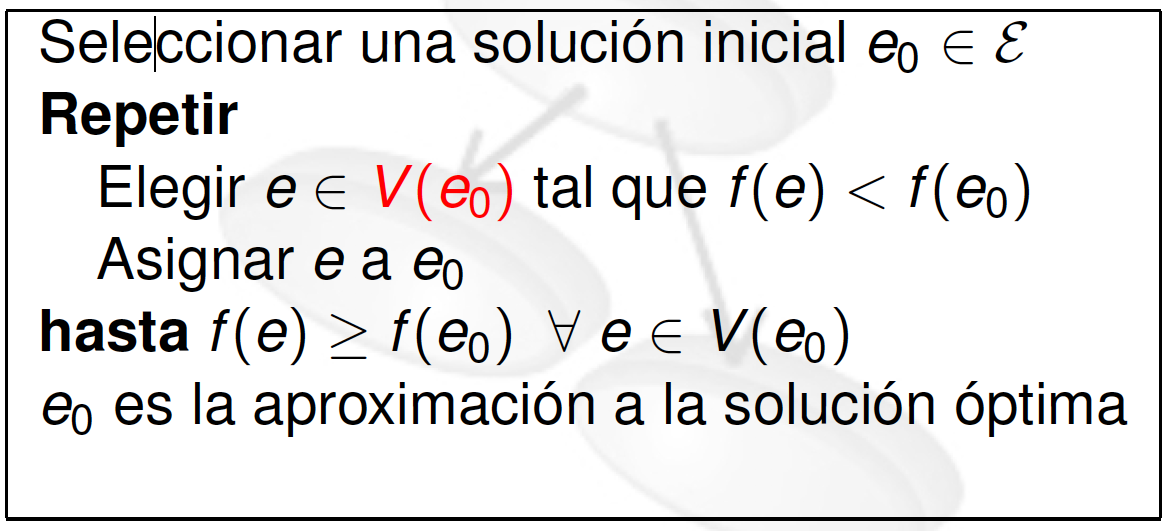
\includegraphics[height=3cm]{/Users/froux/MasterIngeneriaComputacional2018/heuristicosDeBusceada/Semana4/Pseudo-code-for-local-search.png}
 \end{center}
 
 Basicamente, la busquéda local empieza con una solución inicial y busca en su vecindad una mejor solución. Si la solución encontrada es mejor que la solución acutal, la solución acutal es remplazada por la encontrada y continua el proceso, hasta que no se puede mejorar la solución actual. Merece destacar que el diseño de la vecindad es crucial para el desempeño de la busquéda local (y de muchos otros algoritmos de otimización). \newline
 
 La ventaja principal de la busquéda local es de encontrar soluciónes rapidamente, mientras que su principal desventaja es que queda fácilmente en mínimos locales y que su solución final depende de la solucíon inicial. Dado una misma entrada, la busquéda local regresa siempre a la misma salida, propiedad que se puede ver como un pozo de atracción.

 
 \subsection{Multiarranque y búsqueda local para QAP}
El diseño de la vecindad  y el método mutiarranque en el trabajo presente ha sido implementado según el pseudo-codigo siguiente:\newline
 
  \begin{center} 
 \includegraphics[height=10cm]{/Users/froux/MasterIngeneriaComputacional2018/heuristicosDeBusceada/Semana4/Pseudo-code-for-multistart.png}
 \end{center}
 
 \subsection{GRASP y búsqueda local para BIPART}
  Falta de tiempo.
  
  \section{Propuestas de solución basadas en algoritmos poblacionales}
  A continuación se describe el enfoque elegido en este trabajo para resolver los problemas QAP y BIPART mediante algoritmos poblacionales.
  En los dos casos se utilizo el algoritmo genético simple con diferentes operadores de cruce, de mutación y de selección. 

 \subsection{QAP y algoritmo genetico simple}  
 Para resolver el problema QAP se utilizo un operador de cruce de correspondencia parcial (PMX). Con este operador una parte de la rista representando a un padre se hace corresponder a otra parte, de igual tamaño, a la ristra del otro padre, intercambiándose la información restante. Por ejemplo, si consideramos las dos soluciones del problema QAP siguientes: (1 2 3 4 5 6 7 8) y (3 7 5 1 6 8 2 4) el operador PMX crea las ristras de los descendientes de manera siguiente:\newline\newline
 1) Selección con probabilidad uniforme de dos puntos de corte en las ristras de los padres. \newline
 2) Se establece una correspondencia biunívoca entre los elementos que forman parte de las subristas comprendidas entre los puntos de corte.\newline
 3) La subrista del primer padre se copia en el segundo hijo, y de forma análoga, la subrista del segundo padre se copia en el primer hijo.\newline
 4) Cada i-ésimo descendiente se rellena copiando elementos del i-ésimo padre, teniendo en cuenta la correspondecias biunivocas.\newline\newline
 Aplicando estos pasos obtenemos el descendiente 1 y el descendiente 2 para el ejemplo dado:.\newline\newline
 1. (1 2 3 $\mid$ 4 5 6 $\mid$ 7 8) y (3 7 5 $\mid$ 1 6 8 $\mid$ 2 4)\newline
 2. 1$=$ 4, 8$=$6, 6$=$5\newline
 3. (x x x $\mid$ 1 6 8 $\mid$ x x) y (x x x $\mid$  4 5 6 $\mid$ x x)\newline
 4. (4 2 3 $\mid$ 1 6 8 $\mid$ 7 5) y (3 7 8 $\mid$ 4 5 6 $\mid$ 2 1) \newline
 
 Por otro lado, en este trabajo se ha utilizado el operador de mutación mutShuffleIndexes para resolver el problema QAP.
 El operador mutShuffleIndexes funciona de la manera siguiente:\newline\newline
 1. Se fija un probabilidad $p$ de mutación para la población. \newline
 2. Selección aleatoria de un valor $x$ entre 0 y 1 para cada descendiente. \newline
 3. Si $x$ > $p$ se permuten los elementos de una ristra de manera aleatoria.\newline
 
 Finalmente, se ha utilizado la selección por torneo para evolucionar la población. En la selección por torneo se escogen al azar un número $k$ (tamaño del torneo) de individuos de la población y se seleciona el mejor individuo de este grupo. El proceso se repite hasta que el número de individuos seleccionados esta igual al tamaño de la población original.
  
 \subsection{BIPART y algoritmo genetico simple}
 Falta de tiempo.
 
  \section{Experimentos}
Creo haber observado que para el problema BIPART, el algoritmo genetico produce fluctuaciones para pequeñas valores del tamaño del torneo. A continuación se muestren los resultados obtenidos con el algoritmo genético simple para el problema BIPART con tamaño de torneo k=2 y k=10 y los operadores de cruce en dos puntos y de mutación mutFlipBit.

  \begin{center} 
 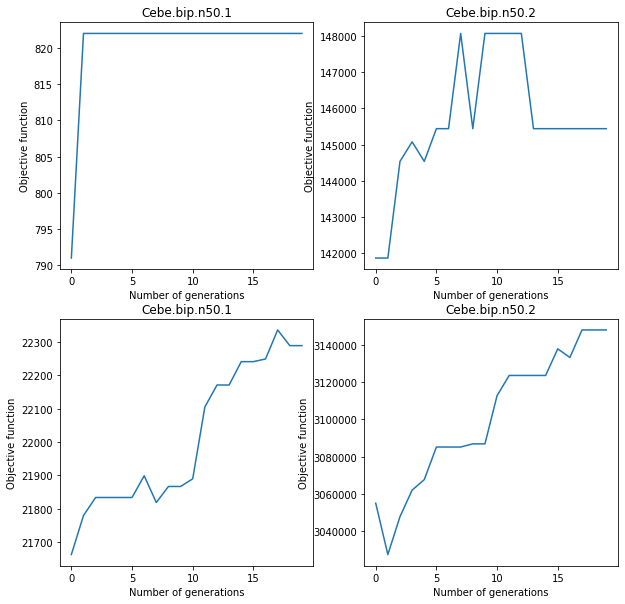
\includegraphics[height=10cm]{/Users/froux/MasterIngeneriaComputacional2018/heuristicosDeBusceada/Semana4/torneo2.png}
 \end{center}


  \begin{center} 
 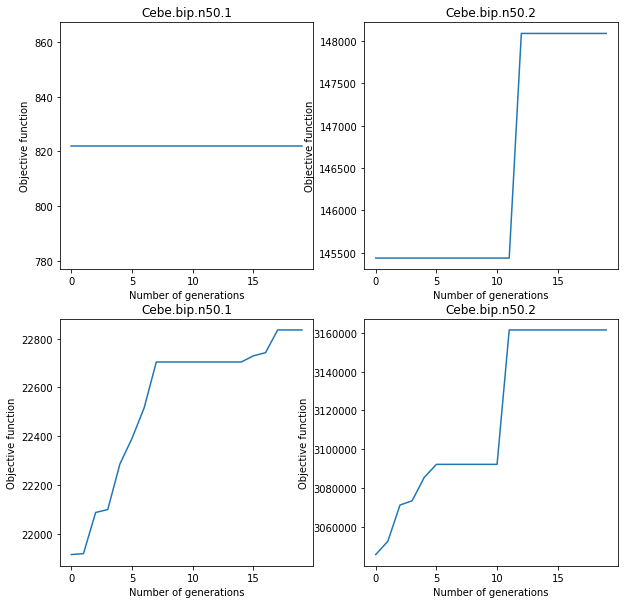
\includegraphics[height=10cm]{/Users/froux/MasterIngeneriaComputacional2018/heuristicosDeBusceada/Semana4/torneo10.png}
 \end{center}
 
 \section{Referencias}
[1] Cormen TH., \& Cormen, TH. (2001). Introduction to Algorithms. Cambridge, Mass: MIT Press. \newline\newline
[2] Gendreau M. \& Potvin JY. (2010). Handbook of Metaheuristics. Springer. \newline\newline
[3] Feynman R. (1982), Simulating Physics with Computers, Int’l J. Theo-retical Physics, 21(6-7):467-488.\newline\newline
[4] Mertens S. (2002), Computacional Complextiy for Physicists, Computing in Science \& Engineering, 4(3):31-47.\newline\newline
[5] Anstreicher KM. (2003), Recent Advances in the Solution of Quadratic Assignment Problems. Mathematical Programming Series B, 97:27-42.\newline\newline
[6] Koopmans TC. \& Beckmann MJ. (1957), Assignment Problems and the Location of Economic Activities. Econometrica, 25:53-76. \newline\newline
[7] Hayes B. (2002), The Easiest Hard Problem, American Scientist, 90(2):113-117.\newline\newline\newline\newline
\end{document}